% Exercise ID: MAT_A12OTIMI_ESTU_MPU_001
% Module: Módulo A12 - Otimização | Concept: Estudo da Monotonia
% Type: monotonia_pura | Difficulty: 2/5
% Tags: monotonia, gráfico, ramos, linear
% Author: Professor | Date: 2025-11-26

\exercicio{
Considere o gráfico seguinte, que representa uma função $f(x)$ definida por ramos no intervalo $[0,2]$:

\begin{center}
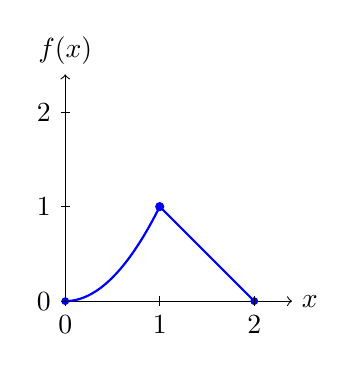
\begin{tikzpicture}[scale=1.2]
  \draw[->] (0,0) -- (2.4,0) node[right] {$x$};
  \draw[->] (0,0) -- (0,2.4) node[above] {$f(x)$};
  % ramos
  \draw[thick, blue, domain=0:1, samples=50] plot (\x, {\x*\x});
  \draw[thick, blue] (1,1) -- (2,0);
  % pontos
  \filldraw[blue] (0,0) circle (1pt);
  \filldraw[blue] (1,1) circle (1.2pt);
  \filldraw[blue] (2,0) circle (1pt);
  % marcas x
  \foreach \x in {0,1,2} \draw (\x,0.05) -- (\x,-0.05) node[below] {\x};
  % marcas y
  \foreach \y in {0,1,2} \draw (0.05,\y) -- (-0.05,\y) node[left] {\y};
\end{tikzpicture}
\end{center}
}

% f(x) = x^2 se 0 <= x < 1; f(x) = 2-x se 1 <= x <= 2
% Contexto adaptado: análise de monotonia e extremos de função por ramos quadrático/linear


\subexercicio{Indica os intervalos de $x$ onde $f(x)$ é crescente, decrescente e constante.}

\subexercicio{Qual é o valor máximo e o valor mínimo de $f(x)$ no intervalo $[0,3]$? Em que pontos ocorrem?}

\subexercicio{Interpreta o significado dos diferentes ramos do gráfico.}
